\atstartofhistorysection
\section[Un peu d’histoire : de la turbine à vapeur à la turbine à gaz]{Un peu d’histoire :\onlyamphibook{\\} De la turbine à vapeur\onlyamphibook{\\} à la turbine à gaz}
\label{ch_histoire_turbine}


Au début du \textsc{xx}\ieme siècle, la \vocab{turbine} a remplacé les pistons et cylindres dans tous les moteurs à vapeur. 
Une turbine est une pièce de géométrie complexe, sensible aux imperfections de fabrication, ce qui rend sa construction plus délicate que celle de pistons cylindriques. En contrepartie, on obtient un moteur d’agencement simple, vibrant peu, et plus facile à assembler, entretenir et lubrifier, ce qui permet d’augmenter sa puissance ou de réduire son volume. L’ingénieur anglais \wf{Charles Algernon Parsons} le démontre de façon spectaculaire en 1897 avec la \textit{Turbinia} (\cref{fig_turbinia}), premier navire en son genre et si rapide qu’aucun bâtiment militaire ne parvient à le rattraper. Dix ans plus tard, toute la \textit{Royal Navy} est propulsée avec des turbines.

	\onlyframabook{\begin{figure}}
	\onlyamphibook{\begin{figure}[htc]}%handmade
		\begin{center}
			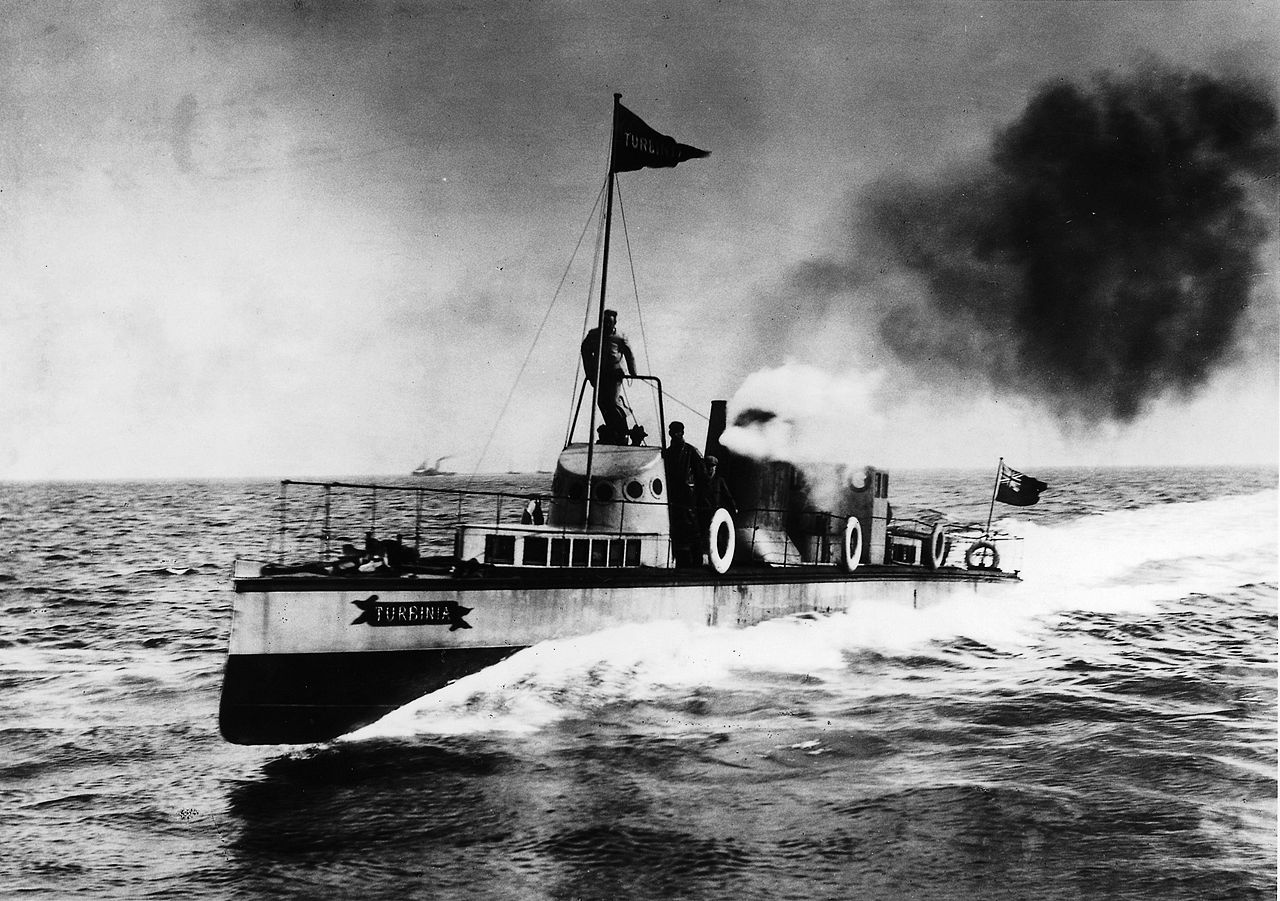
\includegraphics[width=8cm]{images/turbinia.jpg}
			\supercaption{Le \textit{Turbinia}, yatch de Charles Parsons servant de démonstrateur pour ses recherches en propulsion maritime. Avec ses trois turbines à vapeur et ses neuf hélices, il atteint \SI[per-mode=symbol]{60}{\kilo\metre\per\hour} et permet à son propriétaire de ridiculiser la \textit{Royal Navy} pendant le défilé du \textit{Jubilee} de la reine Victoria en 1897.}%
				{\wcfile{Turbinia At Speed.jpg}{photo} par Alfred John West, 1897 (\pd)}
			\label{fig_turbinia}
		\end{center}
	\end{figure}

Dans l’univers des moteurs à gaz, la situation est tout autre : jusqu’à la fin des années 1930, tous les moteurs sont à pistons-cylindres. Cette technologie culmine dans le secteur aéronautique, où l’on arrange les cylindres en étoiles derrière les hélices, pour réduire l’encombrement et les vibrations engendrées. Dans ces machines, telles que le \textit{Twin Wasp} de \textit{Pratt \& Whitney}, l’arrangement mécanique des cylindres, bielles et vilebrequins est absolument phénoménal (\cref{fig_twin_wasp}), et les circuits d’alimentation et de vidange des dizaines de chambres de combustion différentes sont labyrinthiques. Deux ingénieurs, l’allemand \wf{Hans von Ohain} et l’anglais \wf{Frank Whittle}, se consacrent indépendamment à la conception d’un moteur à turbine destiné à s’affranchir de cette complexité.


	\onlyframabook{\begin{figure}}
	\onlyamphibook{\begin{figure}[htc]}%handmade
		\begin{center}
			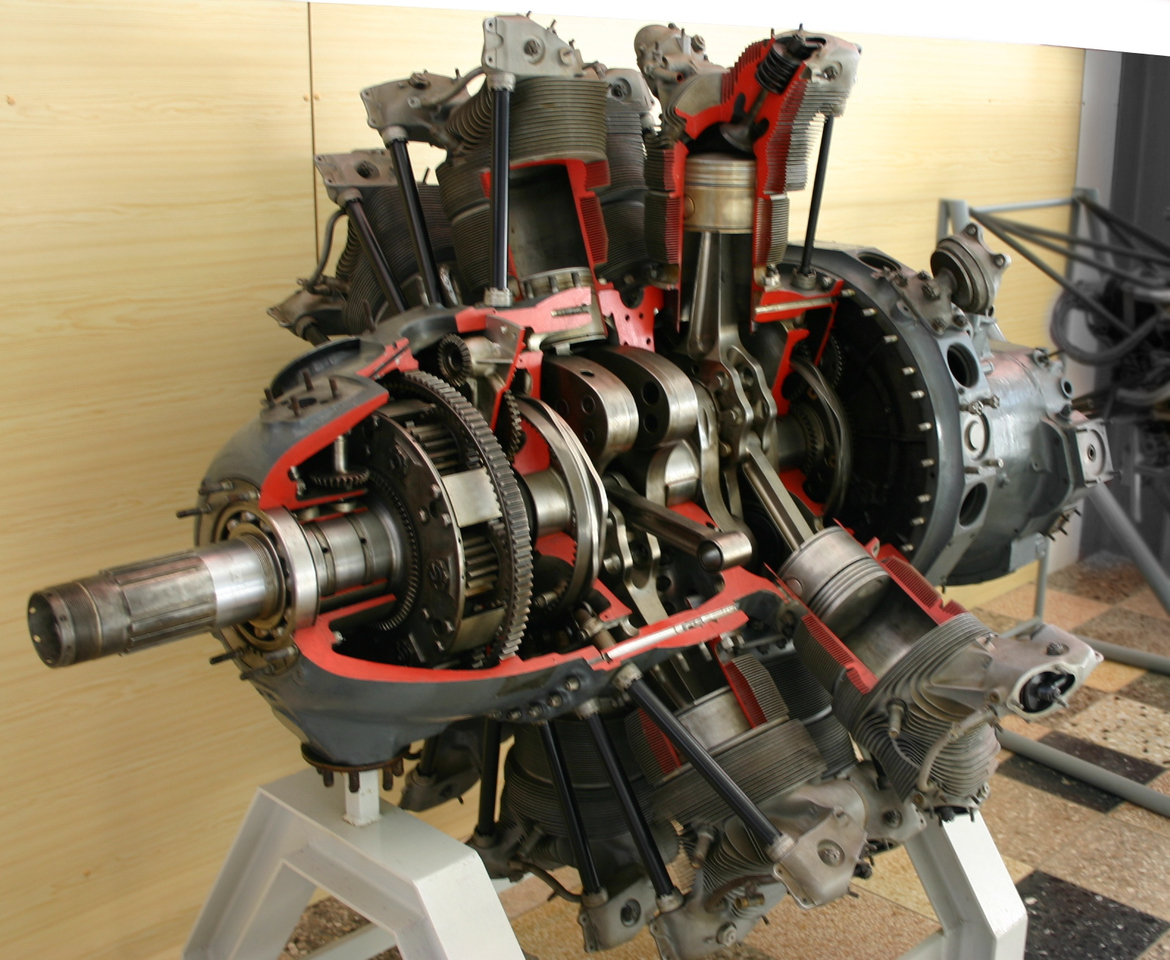
\includegraphics[width=8cm]{images/twin_wasp.jpg}
			\supercaption{Découpe d’un moteur \textit{Pratt \& Whitney Twin Wasp} (1932), montrant l’arrangement intérieur avec bielles et vilebrequins reliant les deux rangées de sept pistons agencés en étoile. Le moteur, de cylindrée \SI{30}{\liter}, dégageait plus de \SI{1000}{ch} et a été produit à plus de \num{170 000} exemplaires.}%
				{photo \ccbysa \olivier}
			\label{fig_twin_wasp}
		\end{center}
	\end{figure}

La mise au point d’un moteur à turbine est bien plus difficile pour les gaz que pour la vapeur. Certes, l’air (ou les gaz brûlés) et la vapeur surchauffée ont des propriétés très similaires : ainsi une turbine à vapeur fonctionne très bien avec de l’air comprimé. La difficulté se trouve à l’autre extrémité du moteur. Dans les moteurs à vapeur la compression de l’eau est faite à l’état liquide, ce qui est très économe. Compresser de l’eau à \SI{10}{\degreeCelsius} de \num{1} à \SI{10}{\bar}, par exemple, ne requiert que $w_\fromatob \approx v_L (p_\B - p_\A ) = \num{0,001} (10 - 1) \times \num{e5} = \SI{900}{\joule\per\kilogram}$ (\ref{eq_pompe_liquide}). Par contraste, faire de même avec de l’air demande une puissance spécifique minimale de $w_\fromatob = c_p \Delta T = c_p \left( T_\A \left(p_\B/p_\A\right)^\frac{\gamma - 1}{\gamma} - T_\A \right) = \num{1005} \left(\num{283,15} \left(10\right)^\frac{\num{0,4}}{\num{1,4}} - \num{283,15} \right) = \SI{265}{\kilo\joule\per\kilogram}$ (\ref{eq_gp_travail_isentropique_so} \& \ref{eq_isentropique_horrible2}), soit presque trois cents fois plus !

Nous avons vu en \S\ref{ch_cycle_de_rankine} que la compression liquide n’est pas sans contrepartie – elle doit être compensée par une plus grande puissance à la chaudière et réduit le rendement thermodynamique — mais elle facilite grandement la mise au point du moteur. Comme la quasi-totalité de la puissance nette du moteur provient de la turbine, une détente peu réversible ou incomplète n’affecte «~que~» la puissance et le rendement du moteur. Dans une turbomachine à gaz, en revanche, la turbine alimente aussi le compresseur : elle joue donc un rôle double. Tant qu’elle ne dégage pas une puissance suffisante pour égaler celle du compresseur, le moteur ne fonctionne pas du tout. L’efficacité isentropique de la turbine et du compresseur deviennent de fait des paramètres primordiaux (nous y reviendrons en \S\ref{ch_rapport_des_puissances} avec la notion de \vocab{marge de travail}) et il s’ensuit que la mise au point de la turbomachine à gaz est une entreprise ambitieuse.


Whittle et Von Ohain vont tous deux concentrer leurs efforts sur un moteur aéronautique ingénieux nommé \vocab{turboréacteur} : ce sont les gaz d’échappement, en grande quantité et avec une forte pression résiduelle, qui vont fournir la poussée du moteur (\S\ref{ch_turboreacteur}). Le principe de fonctionnement est simplissime (le flux d’air est ininterrompu et il n’y a qu’une pièce mobile) mais les défis sont nombreux. Comme une aile d’avion, les pales du compresseur ont tendance à décrocher à faible puissance et dans les phases transitoires, provoquant des variations de débit brutales et destructrices. Dans les chambres de combustion, il faut empêcher la flamme de lécher les parois (ce qui provoquerait leur fonte) ou de se prolonger, en particulier lors des allumages ou rallumages, dans la turbine. Les contraintes de poids nécessitent l’emploi de matériaux légers qui compliquent la fabrication. Les deux ingénieurs conduisent leurs travaux en plein cœur de la seconde guerre mondiale, chacun financé par des budgets militaires, et les premiers avions à réaction volent en 1940. Les appareils de série qui suivent sont délicats d’utilisation, peu réactifs et leur durée de vie en service atteint à peine \SI{20}{\hour}. Ils arriveront trop tard et en nombre trop faible pour affecter le cours du conflit.

	\begin{figure}
		\begin{center}
			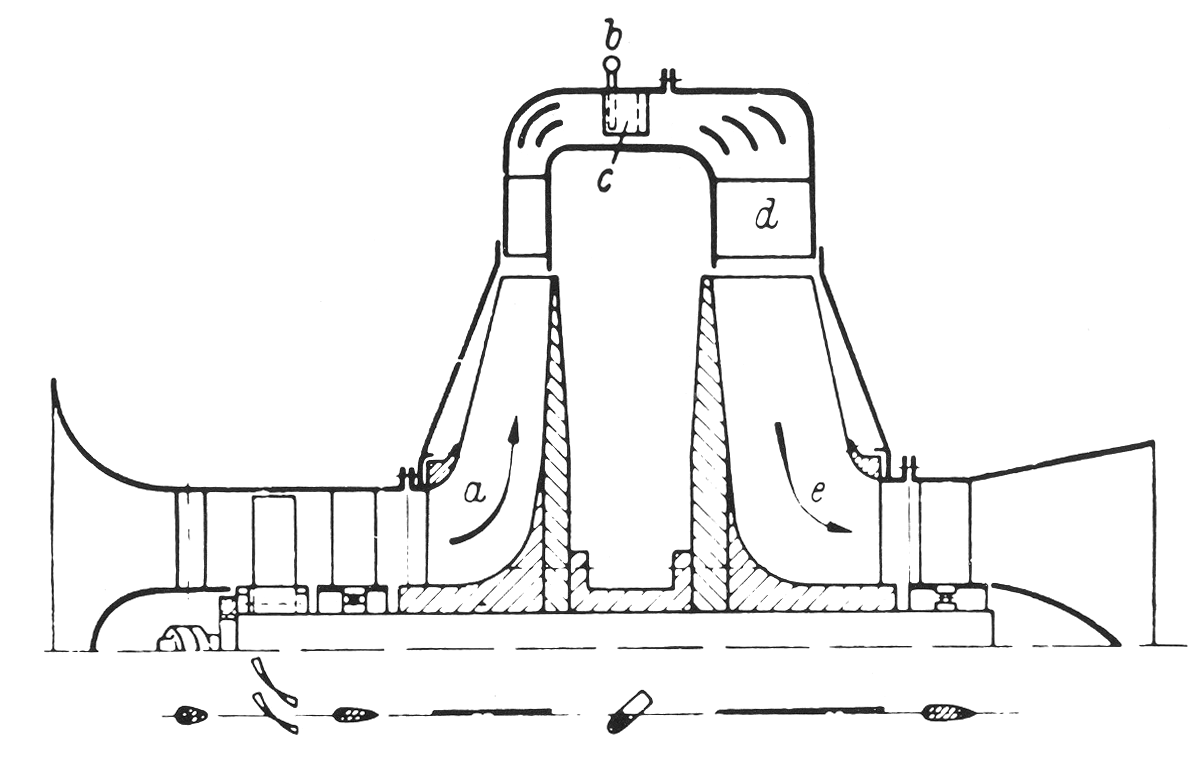
\includegraphics[width=8cm]{images/he_s1.png}
			\supercaption{Schéma de coupe du \textit{Heinkel He S-1}, premier prototype testé par Hans Von Ohain en 1937. Le compresseur est constitué d’un étage axial et d’un étage centrifuge ; la turbine est centripète. Il n’y a qu’une pièce mobile et sa vitesse est uniforme.}%
				{\wcfile{Ohain USAF He S-1 page58.jpg}{schéma} USAF (\pd)}
			\label{fig_turbinia}
		\end{center}
	\end{figure}

À la fin de la guerre, c’est l’engouement : l’aviation s’empare du moteur qu’elle attendait depuis trois décennies. Pour comprendre ce qui fait du turboréacteur le Graal de l’aéronautique du \textsc{xx}\ieme siècle, il faut un peu de mécanique du vol. En vol subsonique, un appareil correctement dessiné a un \vocab{coefficient de traînée} $C_x \equiv F_x \div \left(\frac{1}{2} S_\text{réf.} \rho \ C_\text{vol}^2\right)$ quasi-constant. Ainsi, lorsque l’on réduit la surface alaire $S_\text{réf.}$ et la masse volumique ambiante $\rho$ (en gagnant de l’altitude), on peut augmenter la vitesse de vol $C_\text{vol}$ \emph{en maintenant la traînée $F_x$ constante}. Le coût énergétique du déplacement de l’avion reste alors constant -- en revanche, la puissance à fournir $\dot W_\text{moteur} = F_x C_\text{vol}$, elle, augmente proportionnellement à la vitesse. Ces caractéristiques font des avions des machines relativement économes en énergie, mais très gourmandes en puissance, puisqu’il leur faut maintenir la même poussée à très haute vitesse.

Le turboréacteur a deux atouts pour répondre à ce problème. D’une part, il est compact, léger et sans vibration, ce qui est très désirable pour une application où la traînée (et donc la poussée à fournir) augmente proportionnellement au poids de la machine. D’autre part l’hélice, très efficace en vol lent mais dont les embouts de pale arrivent tôt à des vitesses supersoniques et limitent de ce fait la vitesse des avions, est purement supprimée. Ces deux qualités rendent acceptables les faibles efficacités dues aux compressions et détentes peu réversibles, aux faibles taux de pression et aux vitesses exagérément hautes atteintes par les gaz dans les tuyères.

Ainsi, le gracieux \textit{Lockheed Constellation}, culmination de l’ère de l’aviation à hélice, est rendu instantanément obsolète par l’arrivée en 1949 du \textit{De Havilland Comet}, prodigieux quadriréacteur de même taille mais beaucoup plus rapide (\cref{fig_trois_avions}). Même s’il ne peut initialement franchir la même distance et que sa consommation kilométrique de carburant est plus haute, le \textit{Comet} ne laisse aucune chance à ses concurrents. Sa rapidité est une qualité évidente pour les passagers, mais aussi pour les compagnies dont il augmente nettement la productivité.

	\begin{figure}[htc]
		\begin{center}
			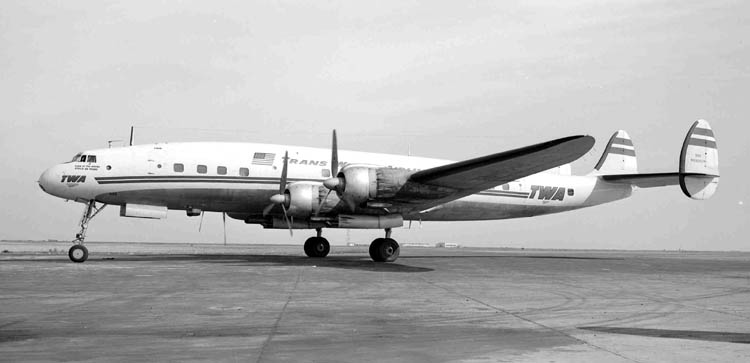
\includegraphics[width=9cm]{images/lockheed_constellation.jpg}
			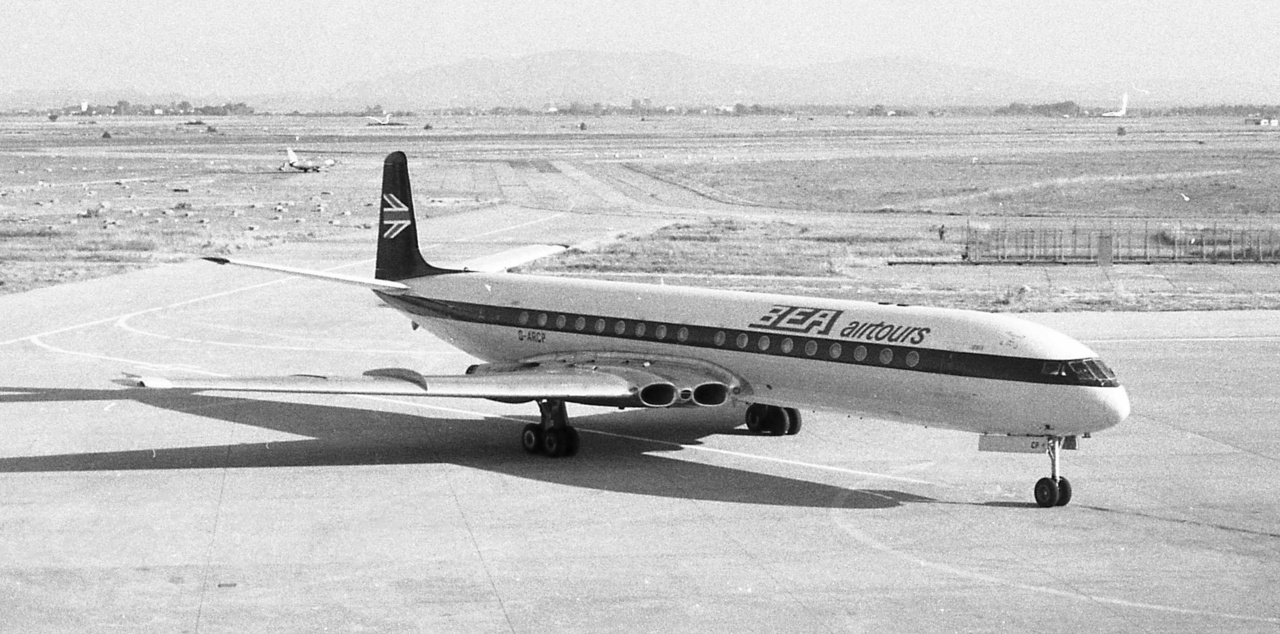
\includegraphics[width=9cm]{images/dhc_comet.jpg}
			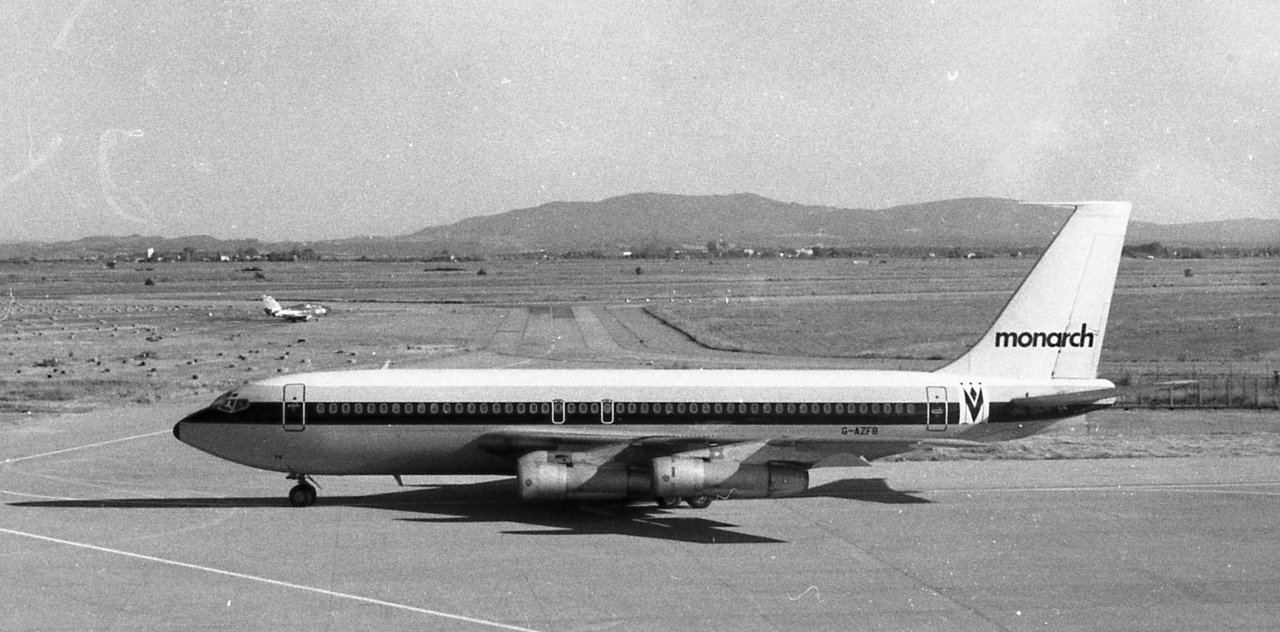
\includegraphics[width=9cm]{images/boeing_707.jpg}
			\supercaption{De haut en bas:\\%
				Le \textit{Lockheed Constellation} (1943), aboutissement de l’ère de l’aviation à hélice : quatre moteurs \textit{Wright Duplex-Cyclone} surcompressés à 18 cylindres chacun, capable de franchir \SI{3700}{\kilo\metre} à \SI[per-mode=symbol]{500}{\kilo\metre\per\hour}.\\%
				Le \textit{De Havilland Comet} (1949), premier avion de ligne à réaction : quatre turboréacteurs \textit{Halford Ghost} monoflux, capable de franchir \SI{2400}{\kilo\metre} à \SI[per-mode=symbol]{740}{\kilo\metre\per\hour}.\\%
				Le \textit{Boeing 707} (1957), dont la configuration et les performances préfigurent celles de tous ses successeurs depuis : quatre turboréacteurs \textit{Pratt \& Whitney JT3C} monoflux, capable de franchir \SI{4300}{\kilo\metre} à \SI[per-mode=symbol]{900}{\kilo\metre\per\hour}.}%
				{\wcfile{Lockheed1049twa (4423687925).jpg}{photo Constellation} \ccbysa par Bill Larkins\\%
				 \wcfile{BEA Airtours Comet G-ARCP 1N.jpg}{photo Comet} et \wcfile{Monarch B-720 G-AZFB 4N.jpg}{707} (retouchées) \ccbysa par Piergiuliano Chesi}
			\label{fig_trois_avions}
		\end{center}
	\end{figure}


Le \textit{Comet}, après la rectification d’un grave défaut de conception, sera lui-même rattrapé par le \textit{Boeing 707} en 1957. Capable de voler plus loin en emportant plus, et encore plus rapide (à \SI[per-mode=symbol]{900}{\kilo\metre\per\hour}, la vitesse que tous les avions de ligne ont adopté depuis, l’air à l’extrados des ailes atteint tout juste la vitesse du son), le \textit{707} marque l’entrée dans l’\textit{ère du jet}, dans laquelle les avions de ligne ne se fabriquent plus par dizaines mais par milliers. Ainsi en vingt-cinq années seulement la turbomachine à gaz a doublé la vitesse des avions et divisé par quatre le prix des billets.
%\onlyamphibook{\pagebreak}%handmade bien pourri, vraiment honteux


%\onlyamphibook{\clearfloats}%handmade
%handmade quote (sur 2 colonnes dans l’amphibook, {quote} est trop étroit
	\onlyframabook{\begin{quote}}
	\onlyamphibook{\begin{historyquote}}
	\begin{footnotesize}
		«~Parés ?~» «~Décollage, top !~» Le mécano pousse avec moi sur les manettes.\\
		NNggnniiiaavvrrooooooaaaaaaarrrrooouuummmmm…\\
		«~N1 vert~». Ça pousse sévère, mais ça accélère tout doucement, étant donné le poids du mastodonte.\\
		«~80 nœuds~» «~Poussée disponible~»\\
		J’ai le bout des pieds sur le palonnier, une précision de tatane similaire à un avion à train classique. Je me régale.\\
		120 nœuds. Au palonnier, je maîtrise, les mecs. 432 passagers et 15 navigants sont accrochés derrière, l’oreille et les sens aux aguets.\\
		140 nœuds. Deux rafales de balises lumineuses défilent sur les côtés. Le palonnier, pointu.
		
		«~V1~» Encore 20 nœuds à prendre pour que l'engin puisse voler. Voilà le bout qui arrive, là-bas devant.\\
		«~Rotation~». À 170 nœuds, je tire doucement, puis plus fermement.\\
		Cinq degrés d'assiette. Dix degrés. Ça s’arrête de rouler, l’aiguille est à 185~nœuds.\\
		Assiette douze degrés. Hue, Cocotte, il faut monter.\\
		«~Vario positif~» «~Train sur rentré~». La vérité se situe ce soir entre douze et treize degrés d’assiette, c'est là que l'aiguille du badin s'immobilise. On passe la côte, et trois-cent pieds en dessous, le passage du \textit{747} doit tenir du séisme.
			\begin{flushright}\vspace{-0.5em}Jacques Darolles, 1998\\ \textit{Le plus beau bureau du monde}~\cite{darolles2000}\end{flushright}
	\end{footnotesize}
	\onlyamphibook{\end{historyquote}}
	\onlyframabook{\end{quote}}

Presque soixante ans après le premier vol du \textit{707}, les avions de ligne volent toujours à la même vitesse, mais la technologie des turboréacteurs n’a cessé de progresser~\cite{rollsroyce2005}. Avec leurs pales de soufflante en composite carbone-époxy ou en titane soufflé, stators de turbine imprimés en céramique, multiples circuits pneumatiques de refroidissement de turbine percés au laser, leurs systèmes électroniques de contrôle, de diagnostic et de surveillance par télétransmission, ils continuent lentement d’augmenter en efficacité. La fiabilité n’est pas en reste : un moteur moderne ne subit en moyenne qu’une défaillance en vol toutes les \num{200 000} heures de vol, et n’est séparé de l’avion pour maintenance que toutes les \num{20 000} heures ou \num{10 000} vols. Un nouveau type de moteur pourra-t-il jamais rendre le turboréacteur obsolète et propulser de nouveau l’aviation vers une nouvelle~ère ?

\atendofhistorysection
